\section{Informação Sensorial: Visão Computacional}

Um veículo móvel terrestre se desloca (geometricamente) apoiado sobre um plano
de suporte, ou seja, seus graus de liberdade usualmente podem ser considerados
em duas dimensões. Desta forma, o reconhecimento do chão representa uma
necessidade e se caracteriza um importante desafio ao se considerar um ambiente
externo não estruturado composto por um solo com vegetação. Além da detecção do
chão, é necessária uma certa classificação das regiões deste plano de suporte
(solo) como sendo, por exemplo, uma superfície transitável ou não transitável:
devido à presença de vegetação, obstáculos, buracos e demais impedimentos.
Os sensores típicos, como sonares e lasers, não apresentam dados muito adequados
para viabilizar essa classificação, uma vez que o sonar possui uma limitação de
alcance e de precisão e o sensor laser de 1 feixe é capaz apenas de analisar uma
seção planar do espaço tridimensional (além de ter um custo muito elevado para
certas aplicações). As câmeras de vídeo são mais adequadas para capturar tais
informações que caracterizam o ambiente, principalmente, se forem usadas câmeras
estéreo, das quais é possível extrair uma informação de profundidade dos
elementos da cena capturada. A utilização de câmeras de vídeo demandam algumas
tarefas elementares, como o ajuste de foco, a utilização de lentes adequadas ao
ângulo de visão necessário e uma devida calibragem. A calibragem das câmeras é
um processo fundamental para se obter um sistema de visão computacional com
representação tridimensional a partir de um par de câmeras independentes
(binocular). Neste processo são calculados (estimados) os parâmetros internos e
externos de cada câmera. Estes parâmetros são essenciais para a reconstrução
tridimensional a partir das imagens capturadas pela câmera estéreo
\cite{Faugeras1993}.

A estimação dos parâmetros internos (intrínsecos) consiste em se obter a
distância focal e o ponto central da imagem, que por questões de alinhamento
entre lentes e sensor pode não ser o pixel central da imagem, influenciando
fortemente os demais processos de estimação \cite{WilsonShafer1994}. Estes
dois parâmetros definem como a imagem é formada por uma câmera estilo
estenopeica (\textit{pin-hole}) e a sua projeção perspectiva. Outros parâmetros
também internos, não associados com o modelo de projeção e sim com as
características físicas das lentes utilizadas, também são estimados no processo
de calibragem. No caso das câmeras de vídeo existe a necessidade de utilização
de lentes, tanto para reduzir a imagem a ser projetada no sensor (filme/CCD)
como para aproximá-las. As lentes comumente são estruturas com curvatura
esférica, característica esta que provoca distorções óticas na imagem projetada.
Estes efeitos são chamados de distorções radiais, produzindo imagens com
demonstrado na \fig{fig:distortions}, nos casos, onde esta distorção pode ser em
forma de “barril” (\textit{barrel}) ou “almofada” (\textit{pincushion})
\cite{Weng1992}.

% (\fig{fig:int_param}).
As distorções óticas influenciam fortemente de forma negativa o processo de
correspondência entre as imagens para extrair a informação tridimensional, sendo
grande fonte de ruído quando não corrigidas. É interessante notar que,
matematicamente, o processo de correção das distorções óticas se baseia na
curvatura esférica da lente, porém as lentes são formadas por uma composição de
várias camadas com curvaturas diferentes (\fig{fig:lens}), que ainda podem
apresentar defeitos no processo de fabricação. Portanto, o modelo matemático
utilizado na correção é sempre uma aproximação global do aparato ótico, fonte
por si só de imprecisão \cite{WilsonShafer1994}.

%Existem ainda outros
%parâmetros que podem ser considerados, porém, estes estão associados a questões
%técnicas da forma de aquisição da imagem e não à formação da imagem propriamente
%dita, portanto são subjetivas ao aparato utilizado sendo necessárias ou não, a
%exemplo, os problemas referentes ao entrelaçamento e varredura da imagem.

% \begin{figure}[ht]
% 	\centering
% 	\begin{minipage}[b]{0.3\linewidth}
% 	    \centering
% 	    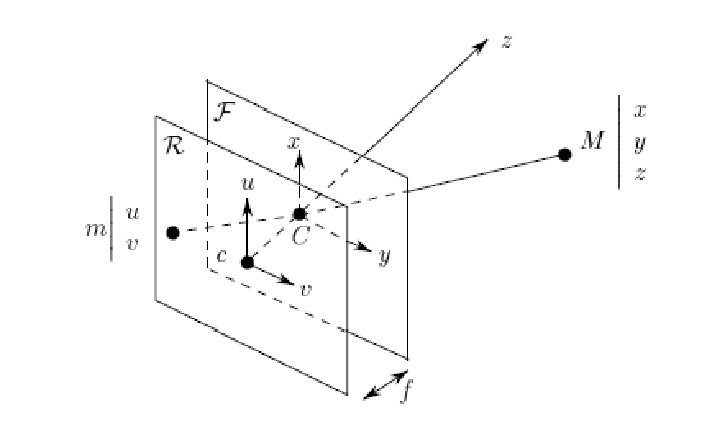
\includegraphics[width=\textwidth]{images/int_param.png}
% 	 	\caption{Ponto central e distância focal}
% 		\fonte{(\cite{Faugeras1993})}
% 	 	\label{fig:int_param}
% 	\end{minipage}
% 	\hspace{0.1cm}
% 	\begin{minipage}[b]{0.3\linewidth}
% 	    \centering
% 	    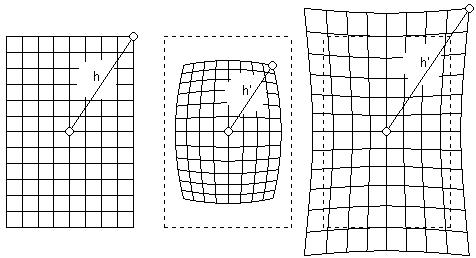
\includegraphics[width=\textwidth]{images/distortions.png}
% 	 	\caption{Distorções óticas}
% 	 	\label{fig:distortions}
% 	\end{minipage}
% 	\hspace{0.1cm}
% 	\begin{minipage}[b]{0.3\linewidth}
% 		\centering
% 	    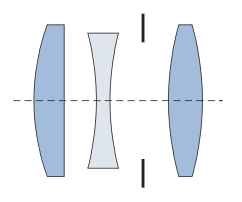
\includegraphics[width=\textwidth,height=3cm]{images/lens.png}
% 	 	\caption{Exemplo de composição ótica}
% 	 	\label{fig:lens}
% 	\end{minipage}
% \end{figure}

\begin{figure}[ht]
	\centering
	\hspace{0.1cm}
	\begin{minipage}[b]{0.45\linewidth}
	    \centering
	    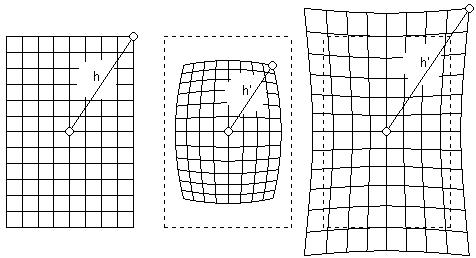
\includegraphics[width=\textwidth]{images/distortions.png}
	 	\caption{Distorções óticas: sem distorção (\textit{esquerda}), 
	 	distorção tipo “barril” (\textif{centro}), 
	 	distorção tipo “almofada” (\textit{direita}).}
	 	\label{fig:distortions}
	\end{minipage}
	\hspace{0.1cm}
	\begin{minipage}[b]{0.45\linewidth}
		\centering
	    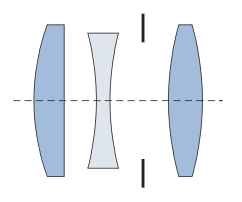
\includegraphics[width=\textwidth,height=4cm]{images/lens.png}
	 	\caption{Exemplo de composição ótica de lentes.}
	 	\label{fig:lens}
	\end{minipage}
\end{figure}


De posse dos parâmetros internos associados às distorções é necessário um
pré-processamento para a sua correção que ao ser aplicado produz uma imagem mais
própria para os algoritmos de correspondência que formarão a imagem
tridimensional. Os parâmetros internos são também chamados de parâmetros do
modelo, isto é, como a imagem é formada. Um outro modelo de câmera geralmente
associado a veículos móveis são as câmeras omnidirecionais, capazes de produzir
uma imagem em 360 graus, útil para veículos com esse grau de liberdade de
movimentos. A calibragem deste tipo de câmera é ainda mais complexa. O segundo
conjunto de parâmetros são os parâmetros externos (extrínsecos), também chamados
de parâmetros de pose. Este conjunto diz respeito à posição da câmera em relação
ao ambiente, no caso, a um sistema de coordenadas referencial. Estes são os
principais parâmetros para a reconstrução tridimensional, pois são utilizados
para se chegar a uma correspondência entre os pixeis de cada uma das duas
imagens. Esta correspondência entre os pontos é obtida pelos princípios da
geometria epipolar (\fig{fig:epipolar}) \cite{Faugeras1993}. De posse dessa
correspondência, a partir do deslocamento destes pontos (disparidade) e um
processo de triangulação, pode ser construída uma representação tridimensional
em um mapa de profundidade. Fundamentalmente, são determinados os planos
formados pelos pontos em comum em cada imagem (referenciais obtidos pela
calibragem) e o ponto central de cada imagem. Esses planos no espaço (ambiente)
são coincidentes, ou seja, o mesmo plano de corte. Esta projeção do plano em
cada imagem definem retas, chamadas retas epipolares. Desta forma é possível
fazer a correspondência dos demais pontos (não referenciais). Este alinhamento
das imagens é chamado de retificação \cite{Fusiello2000}, como pode ser visto
na \fig{fig:rectification}. Pela geometria epipolar todos os planos formados
pelos pontos referenciais serão concorrentes e as suas intersecções se dão em
uma reta em comum, chamada linha base. Esta linha base determina o alcance da
visão (profundidade).

Em um estudo anterior realizado por Klaser \cite{Klaser2007}, em seu trabalho
de conclusão de graduação (TCC), foi aplicada visão tridimensional para
monitorar experimentos de laboratório utilizando como processo de calibragem o
método de Tsai \cite{Tsai1987}. Naquele trabalho, onde as duas câmeras podiam
ser posicionadas em relação ao ambiente com uma certa liberdade observando-se
alguns critérios, foi possível verificar que um conjunto de referenciais capazes
de descrever os três planos ortogonais do espaço tridimensional produziam uma
calibragem bastante precisa. Para isso, foi utilizado um molde semelhante ao
canto de uma sala contendo pelo menos três pontos referenciais em cada parede e
no chão (\fig{fig:bioview}). Uma vantagem do método de Tsai é que o referencial
para a calibragem é dado informando sua posição na imagem e sua posição real no
ambiente, sendo a posição real dada de forma relativa a um sistema de
coordenadas referencial no espaço. Com isso, ao extrair a informação
tridimensional de um ponto pelo processo de triangulação a partir da calibragem
do par estéreo, a informação resultante contém as coordenadas espaciais do ponto
na unidade de medida adotada. Desta forma, é possível saber a posição real de um
determinado ponto, podendo ser extraída uma nuvem de pontos 3D do ambiente
(\textit{3D point cloud}). Porém, para se obter as coordenadas tridimensionais
de um determinado ponto no espaço é necessário saber onde esse ponto se encontra
em cada imagem \cite{MundyZisserman1994}.
Isto não é trivial, mas é possível utilizar métodos de detecção e casamento
(\textit{matching}) de características (\textit{features}) das imagens para
buscar a correspondência, como por exemplo, o método SIFT
(\textit{Scale-Invariant Feature Transform}) \cite{Lowe1999} e o método SURF
(\textit{Speeded Up Robust Features}) \cite{Bay2008}.
% Uma abordagem baseada neste princípio em que, a partir de duas poses da mesma
% cena, se extrai uma terceira coordenada tendo por base uma calibragem das
% câmeras e um processo de correlação global dos pixeis, é chamada de mapa de
% disparidade. Este processo é computacionalmente custoso e existem diversas
% técnicas para a sua implementação.
Uma abordagem para extrair a terceira coordenada espacial tendo por base duas
imagens da mesma cena em poses diferentes e a devida calibragem é chamada de
disparidade \cite{Qian97binoculardisparity}. Este processo é computacionalmente
custoso e existem diversas técnicas para a sua implementação.

\begin{figure}[ht]
	\begin{minipage}[b]{0.3\linewidth}
	    \centering
	    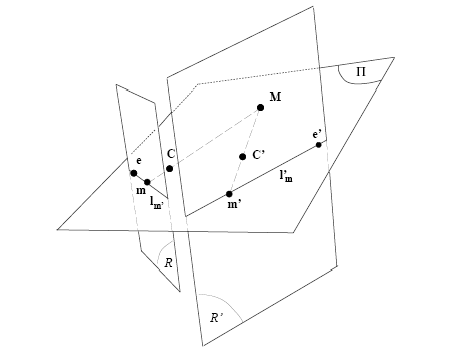
\includegraphics[width=\textwidth]{images/epipolar.png}
	 	\caption{Geometria epipolar}
		\fonte{\cite{Faugeras1993}}
	 	\label{fig:epipolar}
	\end{minipage}
	\hspace{0.1cm}
	\begin{minipage}[b]{0.3\linewidth}
	    \centering
	    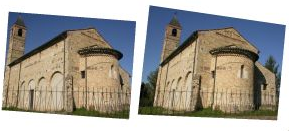
\includegraphics[width=\textwidth,height=4cm]{images/rectification.png}
	 	\caption{Retificação }
		\fonte{Andrea Fusiello}
	 	\label{fig:rectification}
	\end{minipage}
	\hspace{0.1cm}
	\begin{minipage}[b]{0.3\linewidth}
		\centering
	    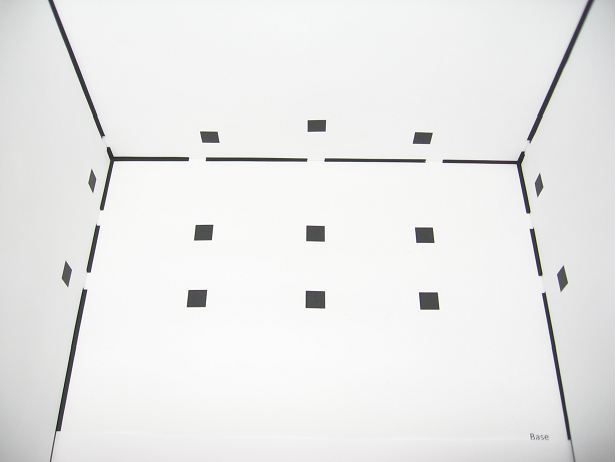
\includegraphics[width=\textwidth,height=4cm]{images/bioview.png}
	 	\caption{Calibragem com referenciais fixos}
		\fonte{\cite{Klaser2007}}
	 	\label{fig:bioview}
	\end{minipage}
\end{figure}

\vspace{0.5cm}


%OSORIO
%> Podia acrescentar uma breve seção sobre GPS:
%2.3 Sensores: Localização e Orientação
%descrevendo sobre a posição (GPS) e orientação (bússola), do veículo e de seu
% destino.
%> O parágrafo abaixo já é uma espécie de "resumo e consolidação" do que foi
%apresentado nas seções anteriores.

Portanto, neste trabalho serão adotados os sensores do tipo GPS e Bússola
(posição e orientação) para localização e câmeras estéreo para a extração de
mapas locais. Estes mapas descreverão o ambiente e os obstáculos através de uma
representação espacial (3D) na qual se encontra o veículo robótico autônomo. A
câmera estéreo irá fornecer um mapa de navegabilidade local composto por
informações obtidas a partir do mapa de disparidade que será descrito a seguir.

%OSORIO
%> Senti falta de uma noção mais geral sobre como passamos da parte de visão
% computacional estéreo para os mapas locais (mapa 3D - cloud of points, mapa local, mapa de navegabilidade). 
% Mapa de disparidade já entra em um conceito específico...
%> Talvez pudesse ter citado o trabalho do Caio (mestrado) e do Patrick
% (mestrado) que tem bons exemplos de mapas (com figuras)  :)


% 2012-10-13 lido OK

